\documentclass[a4paper,11pt]{article}
\usepackage{pos}

\usepackage{caption}
\usepackage{float}
\usepackage[lofdepth=1,lotdepth]{subfig}

\usepackage{wrapfig}

\usepackage{setspace}

\usepackage{braket}

\usepackage[noabbrev, capitalise, nameinlink]{cleveref}  % reference object types automatically

\title{Search for Heavy Neutral Lepton Production and Decay with the IceCube Neutrino Observatory}
\ShortTitle{Search for Heavy Neutral Lepton Production and Decay with IceCube}

\manuallySeparateAuthors
\author*[a]{Leander Fischer}
\author{for the IceCube collaboration}

\affiliation[a]{DESY, D-15738 Zeuthen, Germany}

\emailAdd{leander.fischer@desy.de}

\abstract{
Sterile neutrinos are a well-motivated objective of Beyond Standard Model searches. Extensions to the Standard Model that include right-handed (sterile) neutrinos pose viable explanations for the origin of neutrino masses, and they could also solve a variety of additional open questions in physics, such as neutrino oscillation anomalies, the nature of dark matter, and baryon asymmetry. Multiple models posit the existence of a GeV-scale sterile neutrino (also called heavy neutral lepton), which can interact with the Standard Model particles through mixing. The heavy neutral lepton can therefore be produced from, and decay into known particles. If the production from up-scattering atmospheric neutrinos and the subsequent decay happen inside the IceCube detector, it can produce a unique double-cascade signature. This signature can be utilized to search for GeV-scale heavy neutral leptons at atmospheric neutrino energies. By focusing on the flux of atmospheric muon neutrinos that oscillate into $\nu_\tau$, the less constrained $\tau$-sterile mixing space can be explored. We present an analysis approach to study heavy neutral leptons in the mass range of 0.1\,GeV-2\,GeV, where we search for low-energy double-cascade topologies with the IceCube DeepCore detector.
}

\FullConference{
  41st International Conference on High Energy physics - ICHEP2022\\
  6-13 July 2022\\
  Bologna, Italy
}

\begin{document}
\maketitle


\section{Introduction}

Extensions to the Standard Model (SM) that add heavy neutral leptons (HNLs) provide a good explanation for the origin of neutrino masses through different seesaw mechanisms \cite{10.1143/PTP.64.1103}.
\begin{wrapfigure}{r}{0.5\textwidth}
  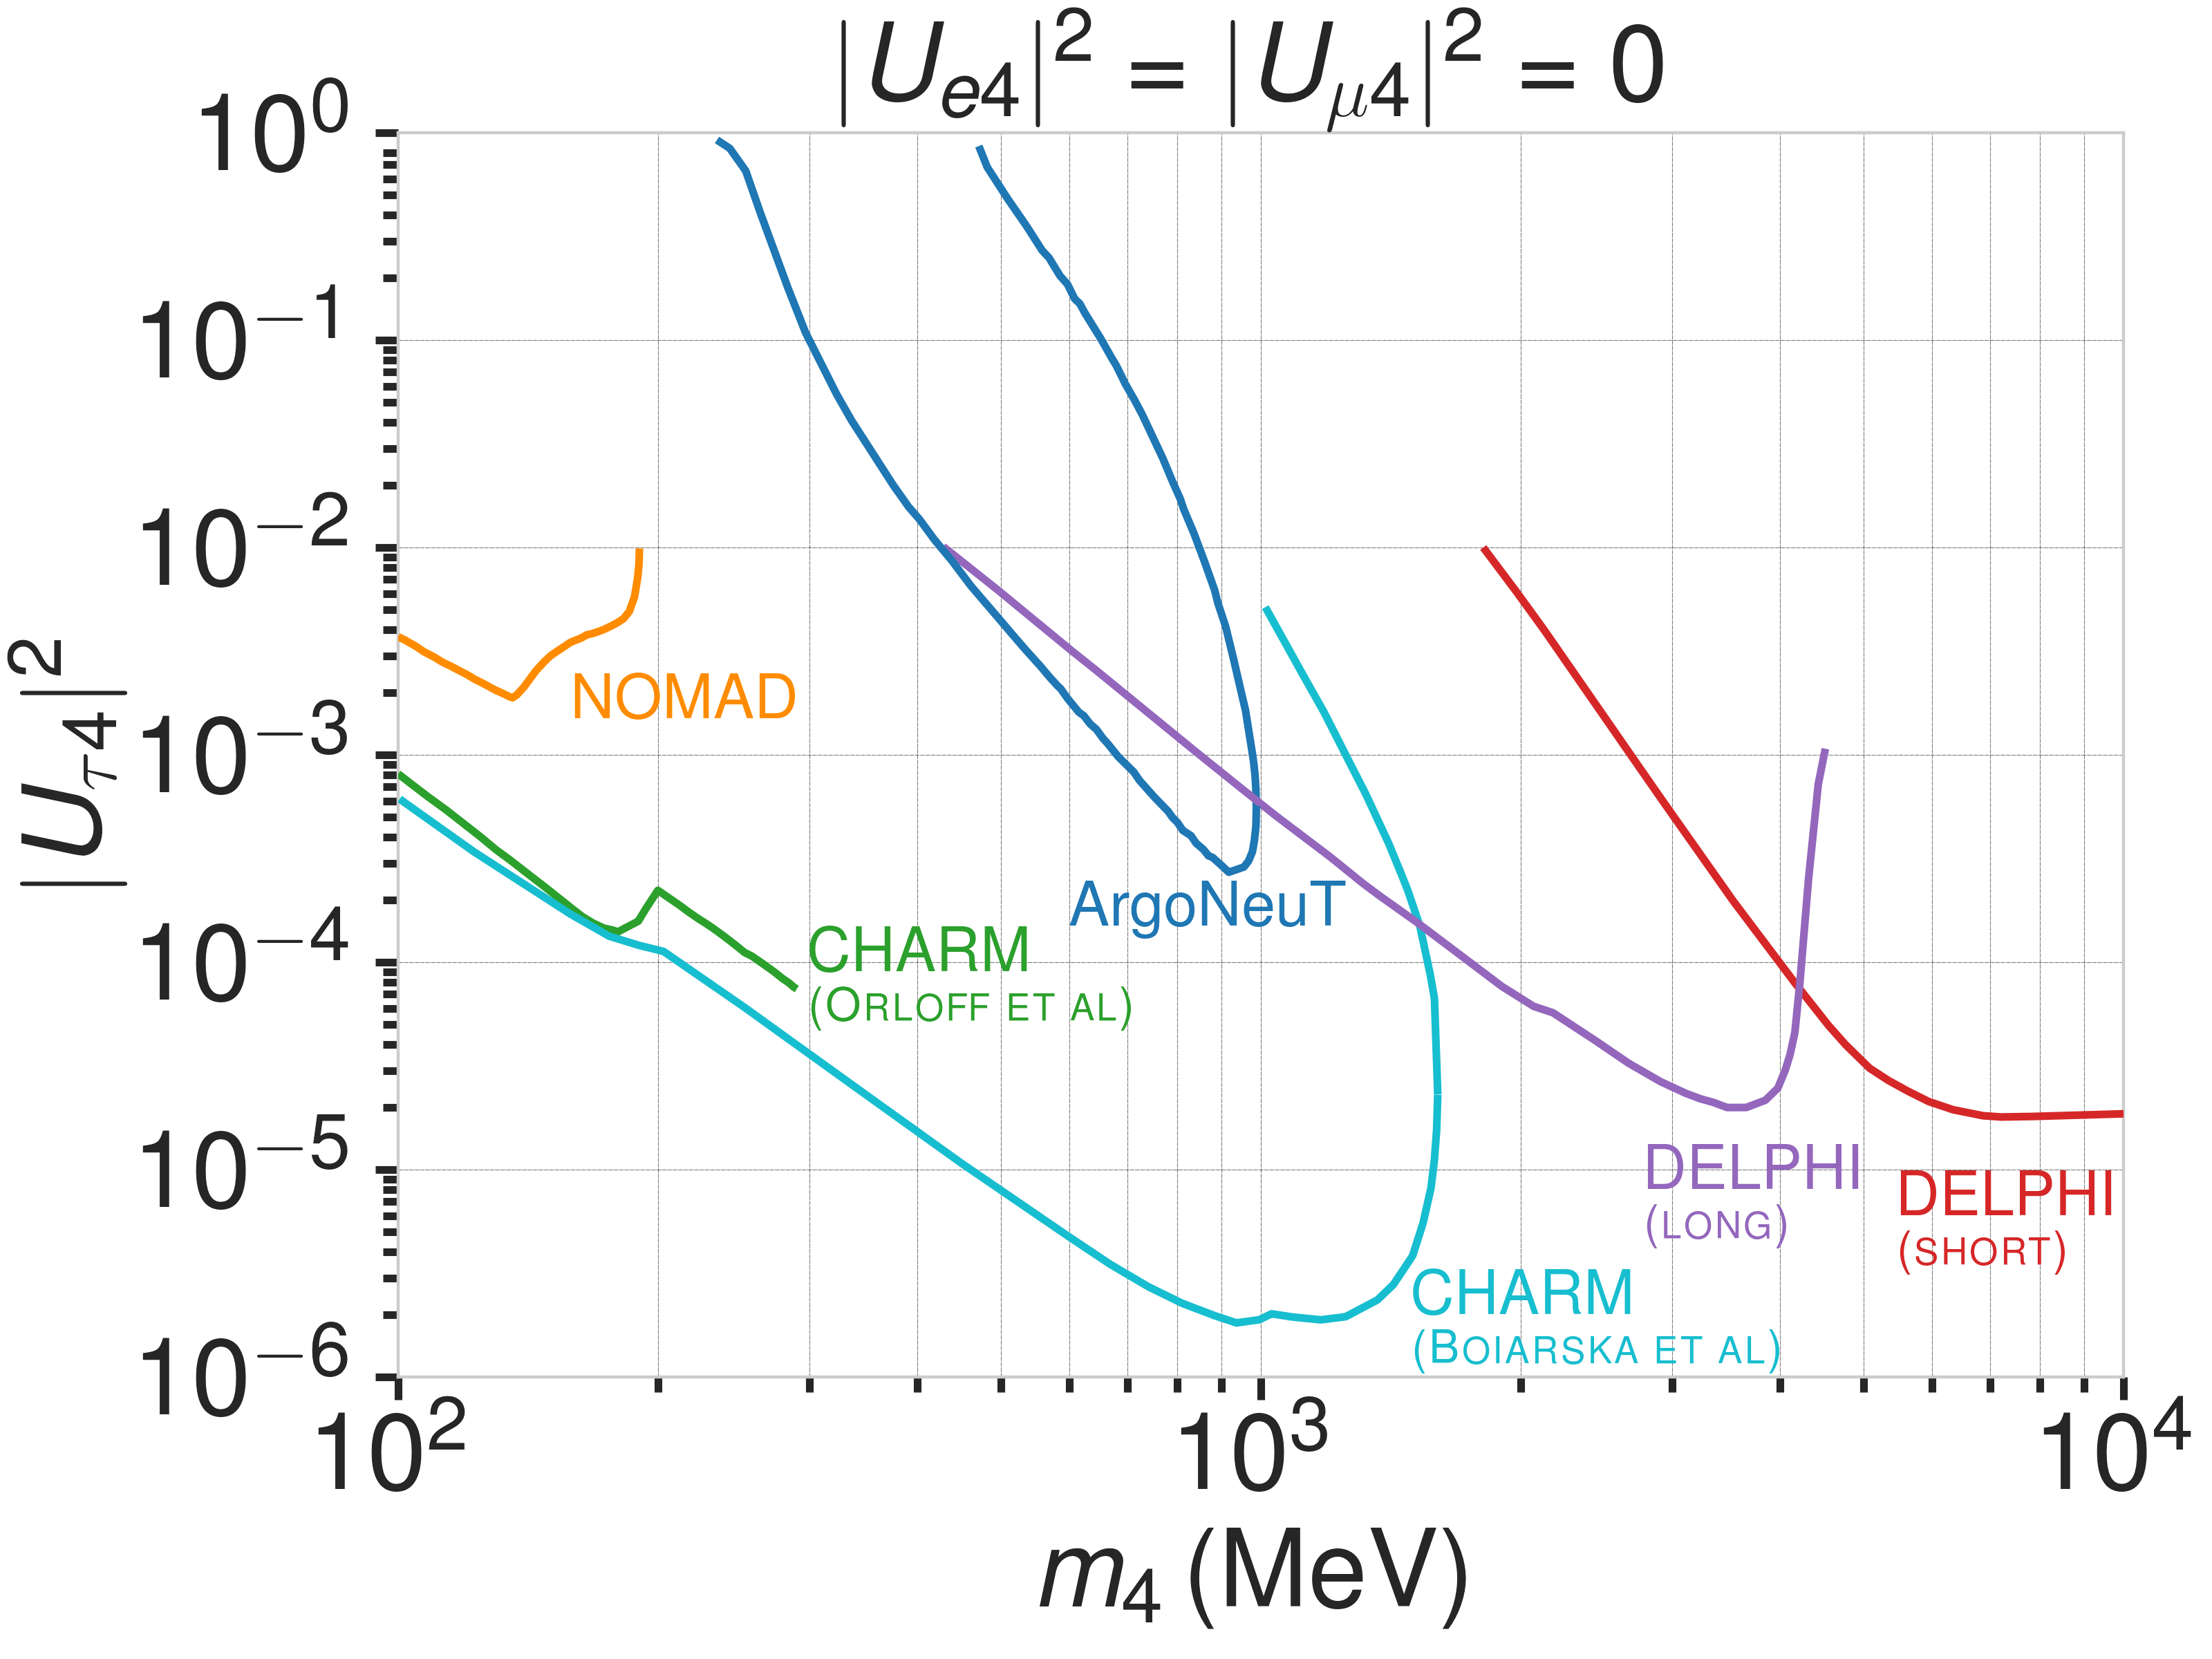
\includegraphics[width=0.5\textwidth]{figures/UtauN_custom_plots_LF_grid_white.png}
  \caption{Current $|U_{\tau4}^2|$ limits from NOMAD \cite{NOMAD:2001eyx}, ArgoNeut \cite{ArgoNeuT:2021clc}, CHARM \cite{Orloff:2002de, Boiarska:2021yho}, and DELPHI \cite{DELPHI:1996qcc}.}
  \label{fig:hnl_limits}
\end{wrapfigure}
While the mixing with $\nu_{e/\mu}$ is strongly constrained ($|U_{\alpha4}^2| \lesssim 10^{-5}-10^{-8}, \alpha=e,\mu$), the mixing with $\nu_{\tau}$ is much harder to probe due to the difficulty of producing and detecting $\nu_\tau$. \cref{fig:hnl_limits} shows the current limits on the $\tau$-sterile mixing for HNL masses between 0.1\,GeV-10\,GeV. As was first pointed out in \cite{Coloma:2017ppo}, the atmospheric neutrino flux observed in IceCube offers a way to constrain the neutrino-HNL mixing parameters. By using the large fraction of atmospheric $\nu_{\mu}$ events that oscillate into $\nu_{\tau}$ before they reach the detector \cite{IceCube:2019dqi}, the less constrained $\tau$-sterile mixing space can be explored.


\vspace{-0.4cm}
\section{IceCube DeepCore}

\begin{figure}[h!]
  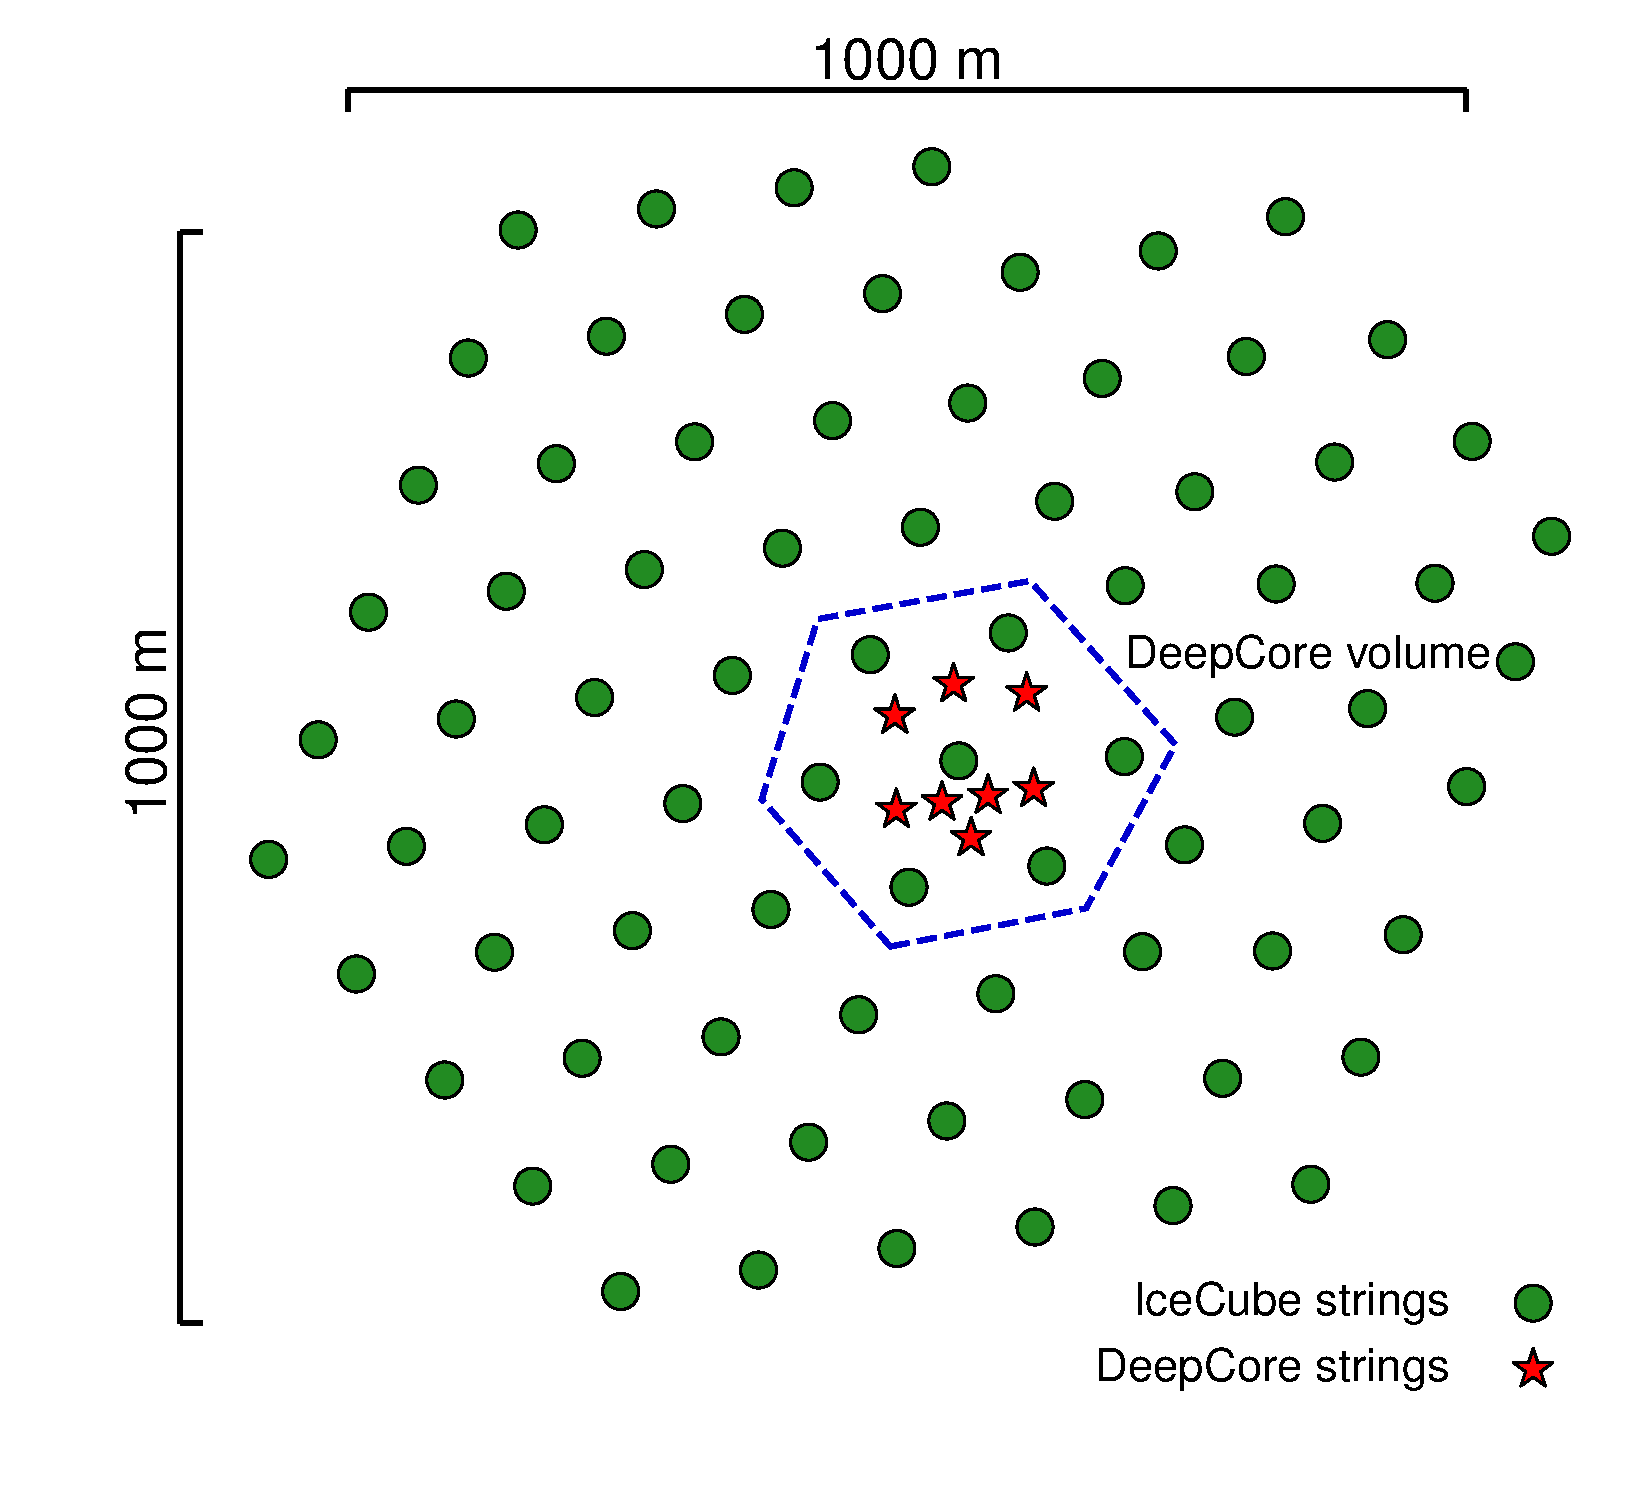
\includegraphics[width=.43\linewidth]{figures/icecube_top_view_bw.pdf}
  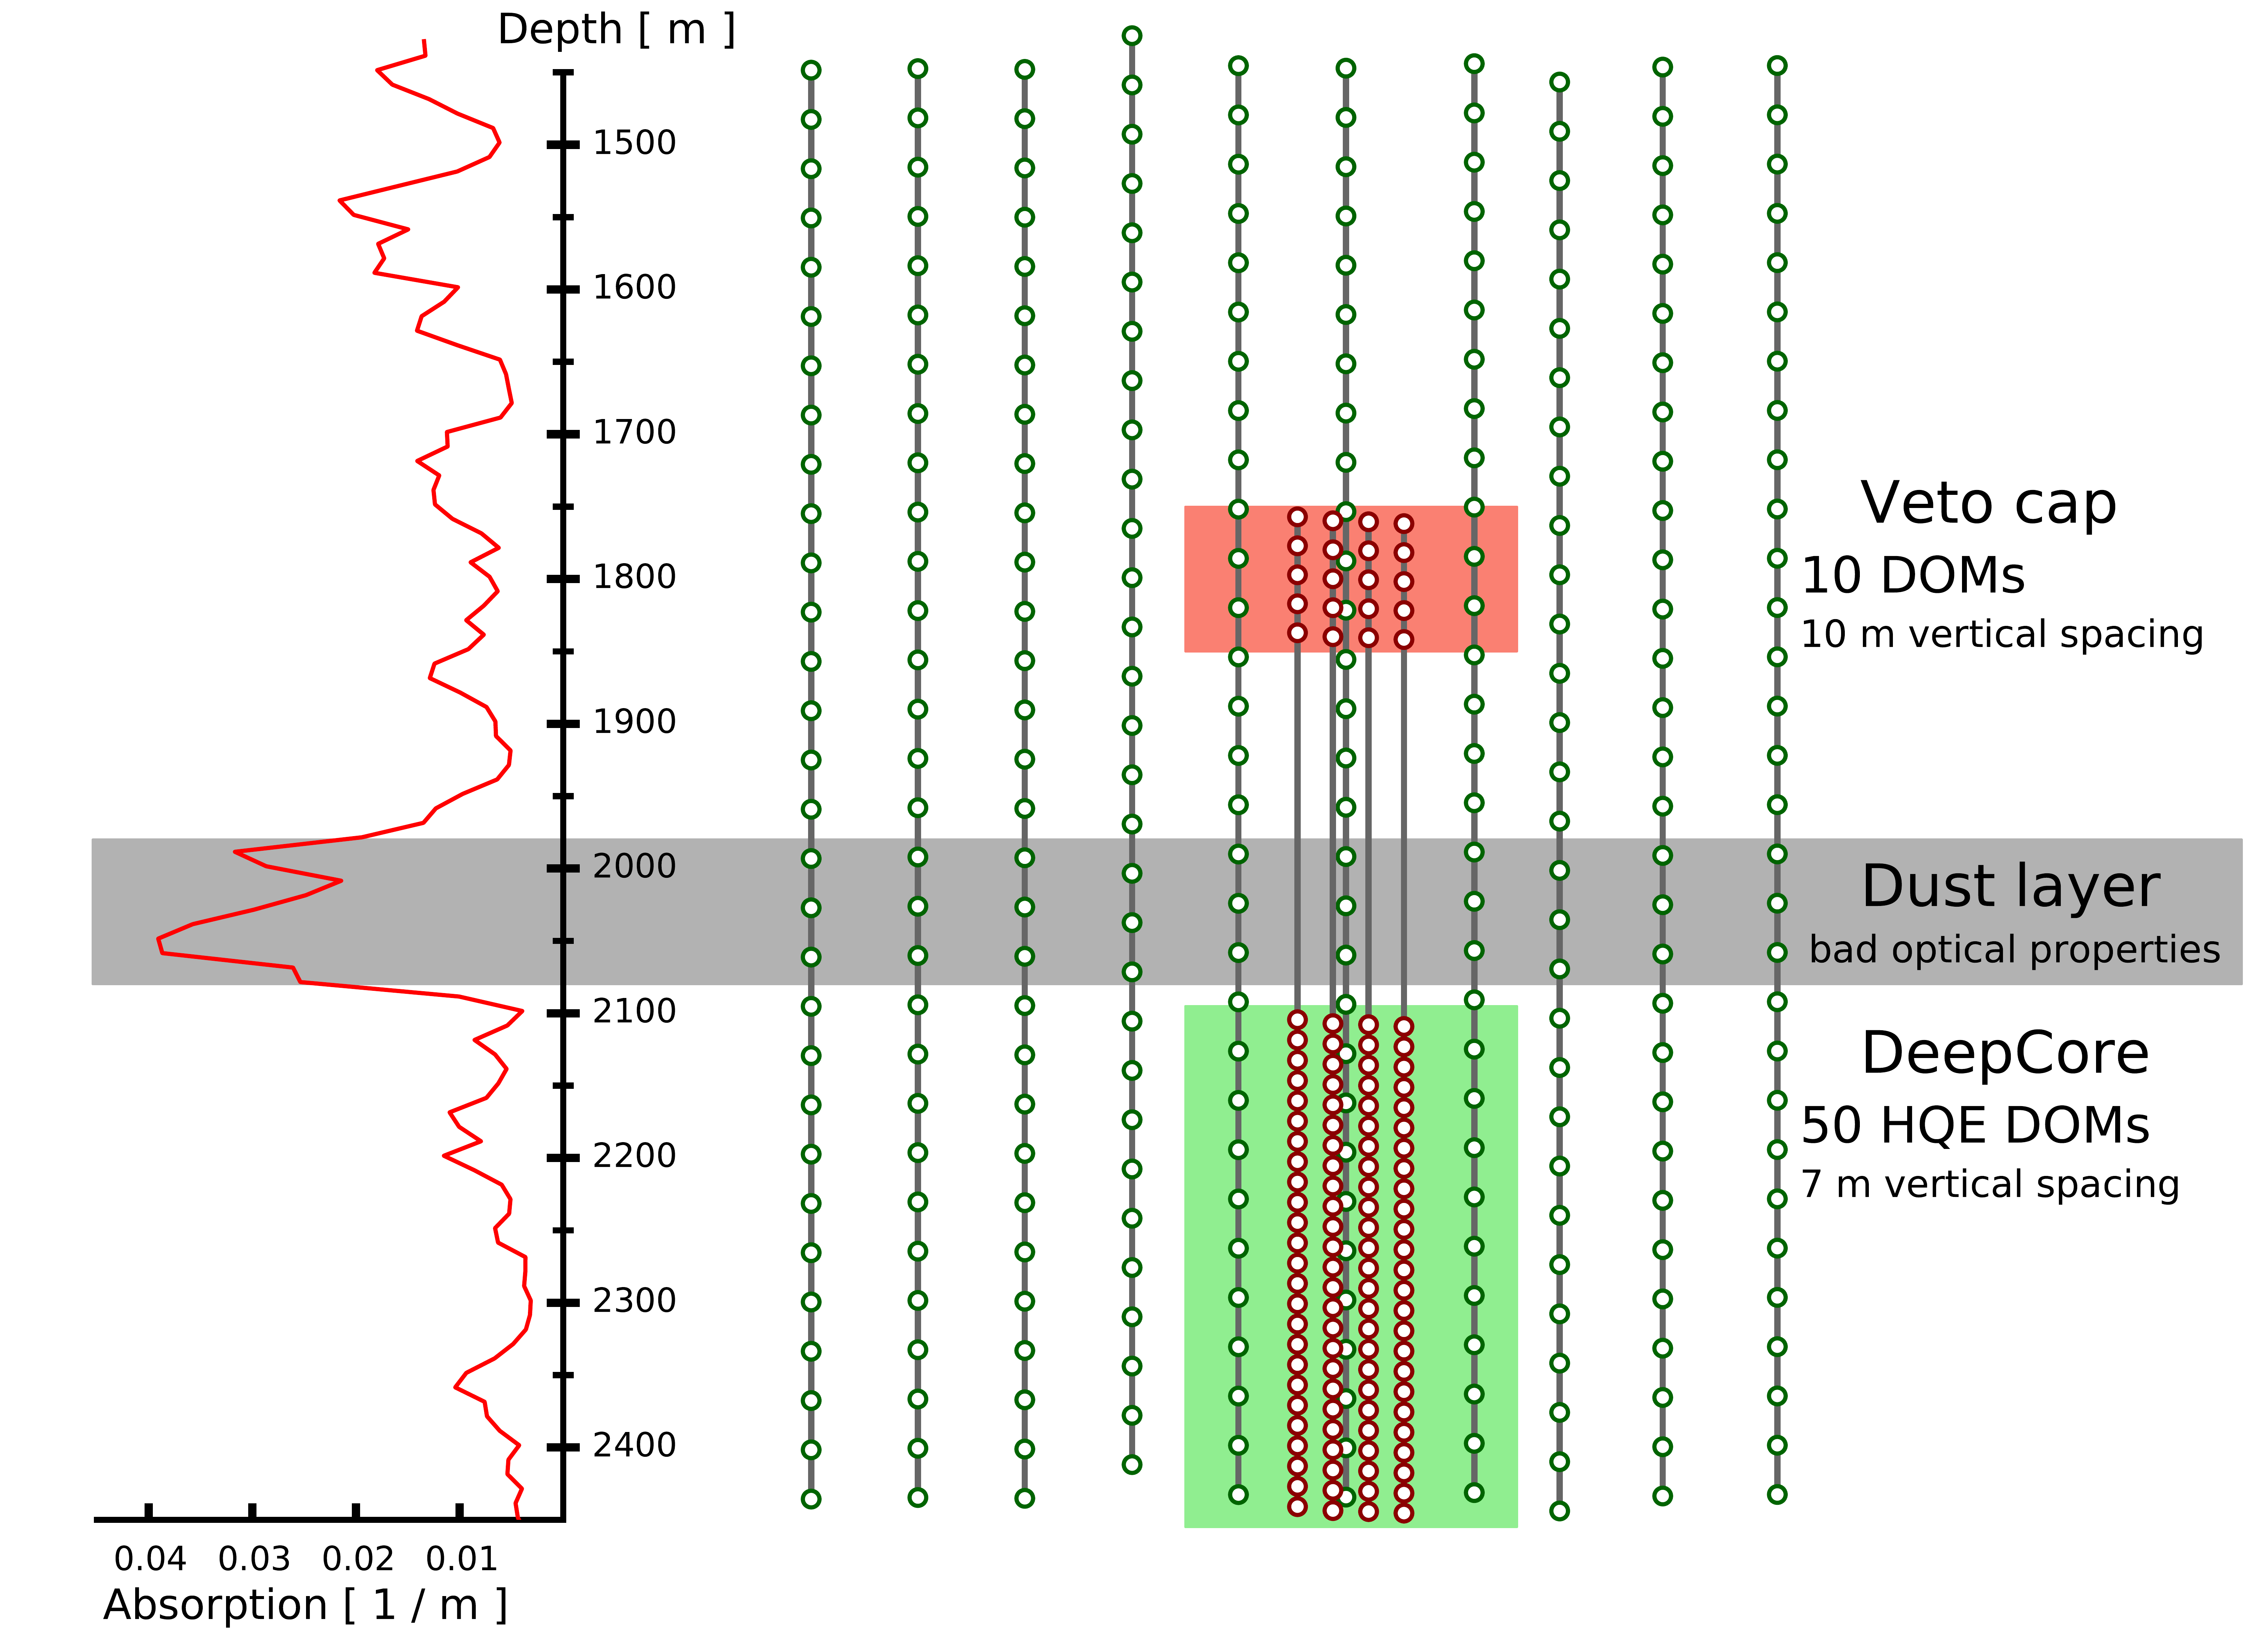
\includegraphics[width=.52\linewidth]{figures/DeepCore_sideview.png}
  \caption{Top-view (left), and side-view (right) of the IceCube and DeepCore array.}
  \label{fig:icecube_array}
\end{figure}

The IceCube Neutrino Observatory \cite{Aartsen:2016nxy} is an ice Cherenkov telescope located at the geographic South Pole. It consists of 5160 Digital Optical Modules (DOMs) deployed into the Antarctic glacial ice at depths between 1.45\,km and 2.45\,km, instrumenting a volume of about 1\,km$^{3}$. The ice is simultaneously the interaction and the detection medium; the interacting neutrinos can produce charged secondary particles, which themselves can emit Cherenkov photons that are detectable by the DOMs. The DOMs are arranged on a nearly-hexagonal array, as shown in \cref{fig:icecube_array}, with 125\,m horizontal and 17\,m vertical spacing in IceCube, and a closer 42-72\,m horizontal and 7\,m vertical spacing in the denser, bottom-center part of the array called DeepCore \cite{IceCube:2011ucd}. While IceCube targets the detection of astrophysical neutrinos with energies above $\sim$100\,GeV, DeepCore can measure neutrino interactions down to a few GeV due to its closer spacing in regions with favorable optical properties of the ice.

\begin{figure}[h!]
    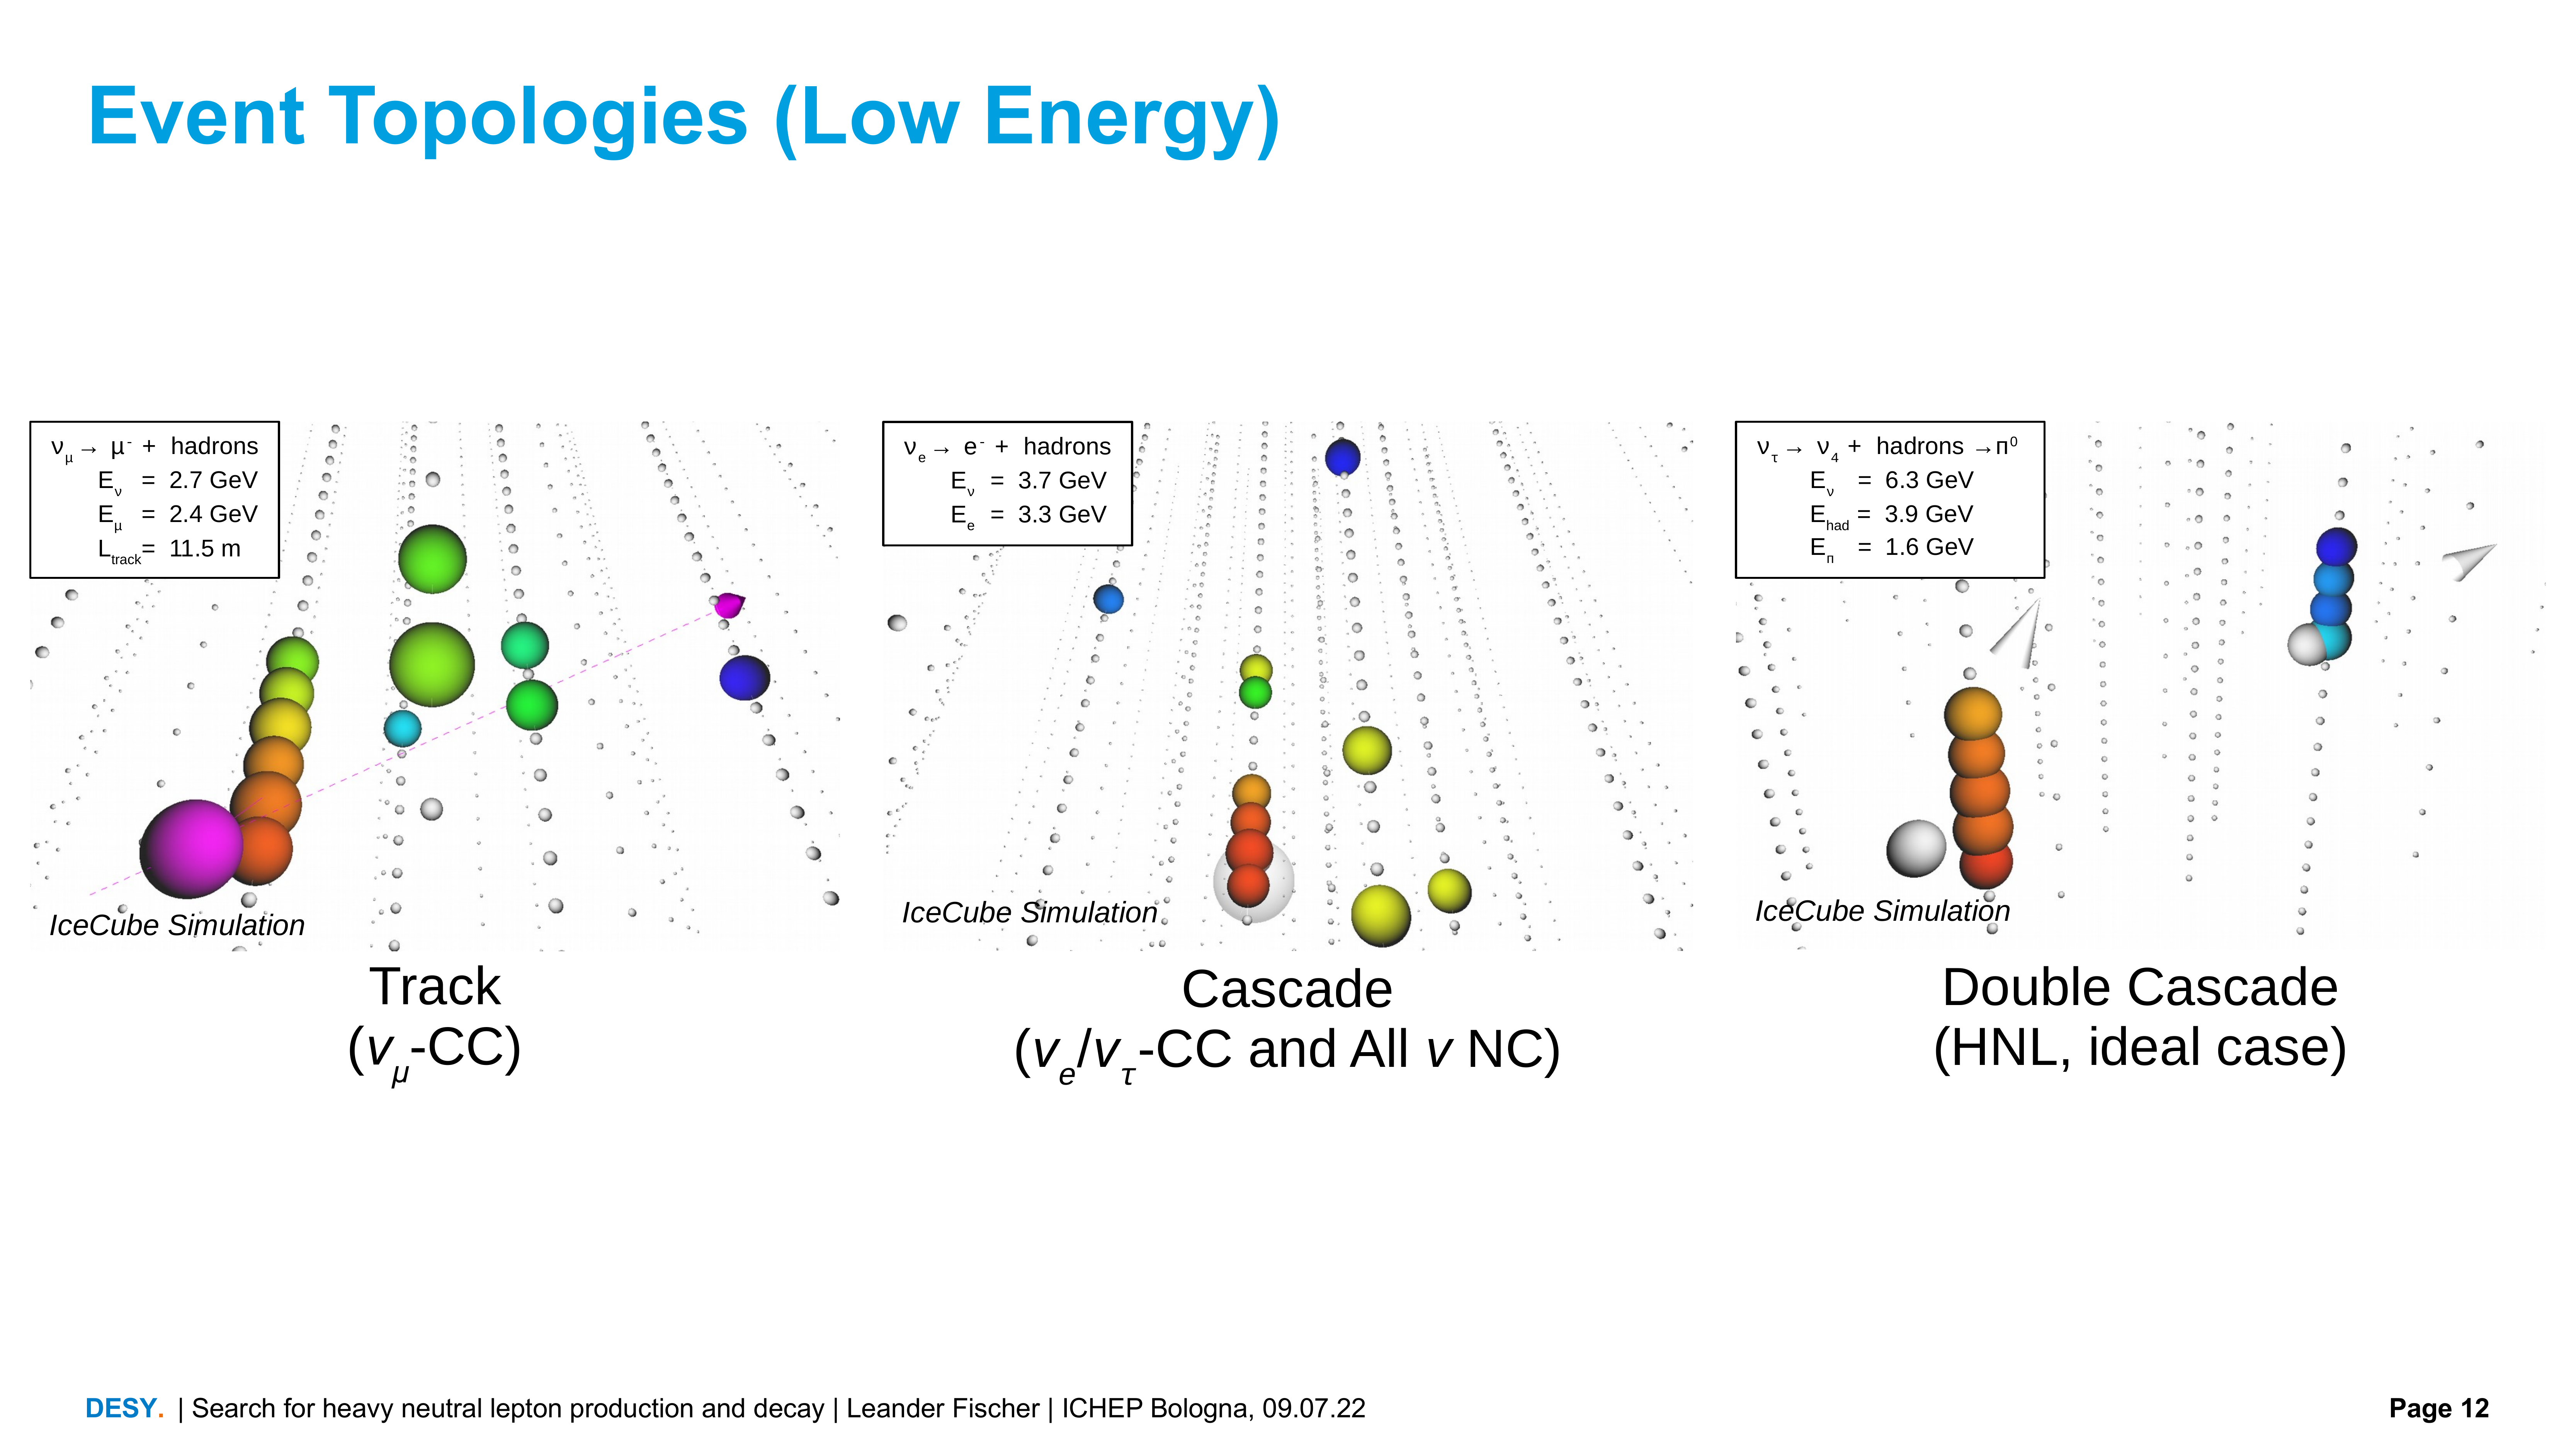
\includegraphics[trim = 0cm 4.5cm 0cm 5.5cm, clip, width=1.0\linewidth]{figures/event_views_all_three.png}
    \caption{Example low-energy event topologies in IceCube. The color of the rainbow spheres indicates the arrival time (red$\rightarrow$blue=early$\rightarrow$late) of the photons, while their size is relative to the detected number. The purple sphere and arrow (left), the grey sphere (middle), and grey spheres with arrows (right) are the positions/directions of the true cascades and tracks.}
    \label{fig:low_energy_eventviews}
  \end{figure}

In the absence of Beyond Standard Model (BSM) physics, the two observable low-energy event topologies in IceCube DeepCore data are \textit{tracks} and \textit{cascades}. Tracks are elongated patterns of light emission that are produced by long-lived muons. These muons mainly originate from $\nu_{\mu}$ charged current (CC) interactions, or cosmic ray air showers, with a subdominant component from $\nu_{\tau}$ CC interactions (Branching Ratio (BR) of $\tau\rightarrow\mu$ $\sim17\,\%$ \cite{PhysRevD.98.030001}). Cascades are roughly point-like, concentrated light emissions, produced by electromagnetic and hadronic showers. They are produced by $\nu_{e}$ CC and most $\nu_{\tau}$ CC interactions, as well as neutral current (NC) interactions of all flavors. \cref{fig:low_energy_eventviews} (left and middle panels) show examples of track-like and cascade-like topologies at atmospheric energies.


\vspace{-0.4cm}
\section{Neutrino Oscillations in the 3-Neutrino Framework} \label{sec:neutrino_oscillations}

\begin{figure}[h!]
  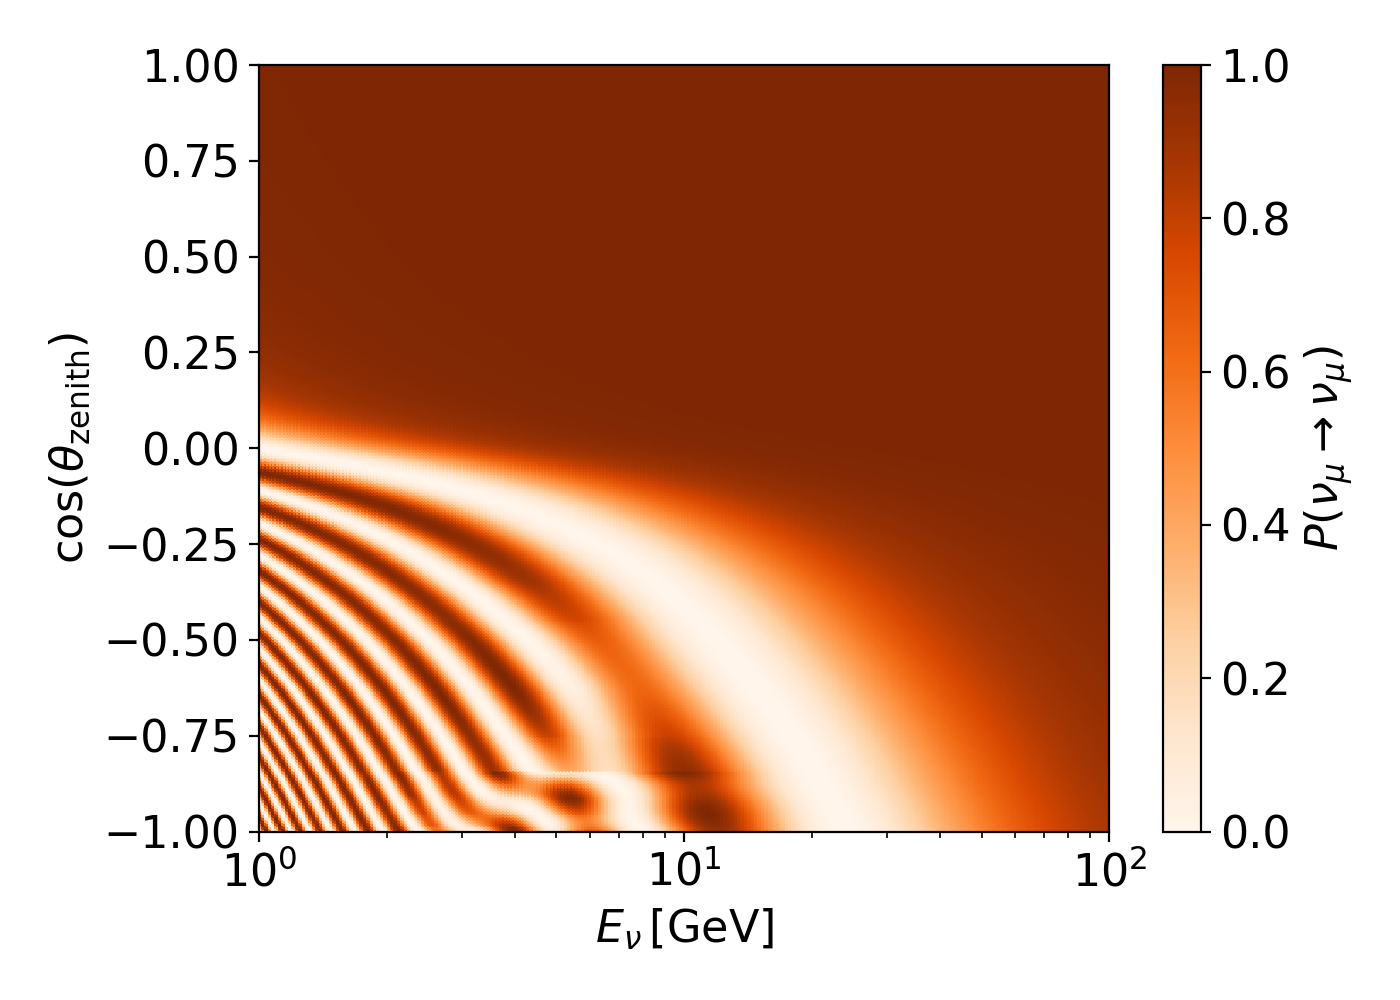
\includegraphics[width=.44\linewidth]{figures/Oscillogram_numu_numu_orange.png}
  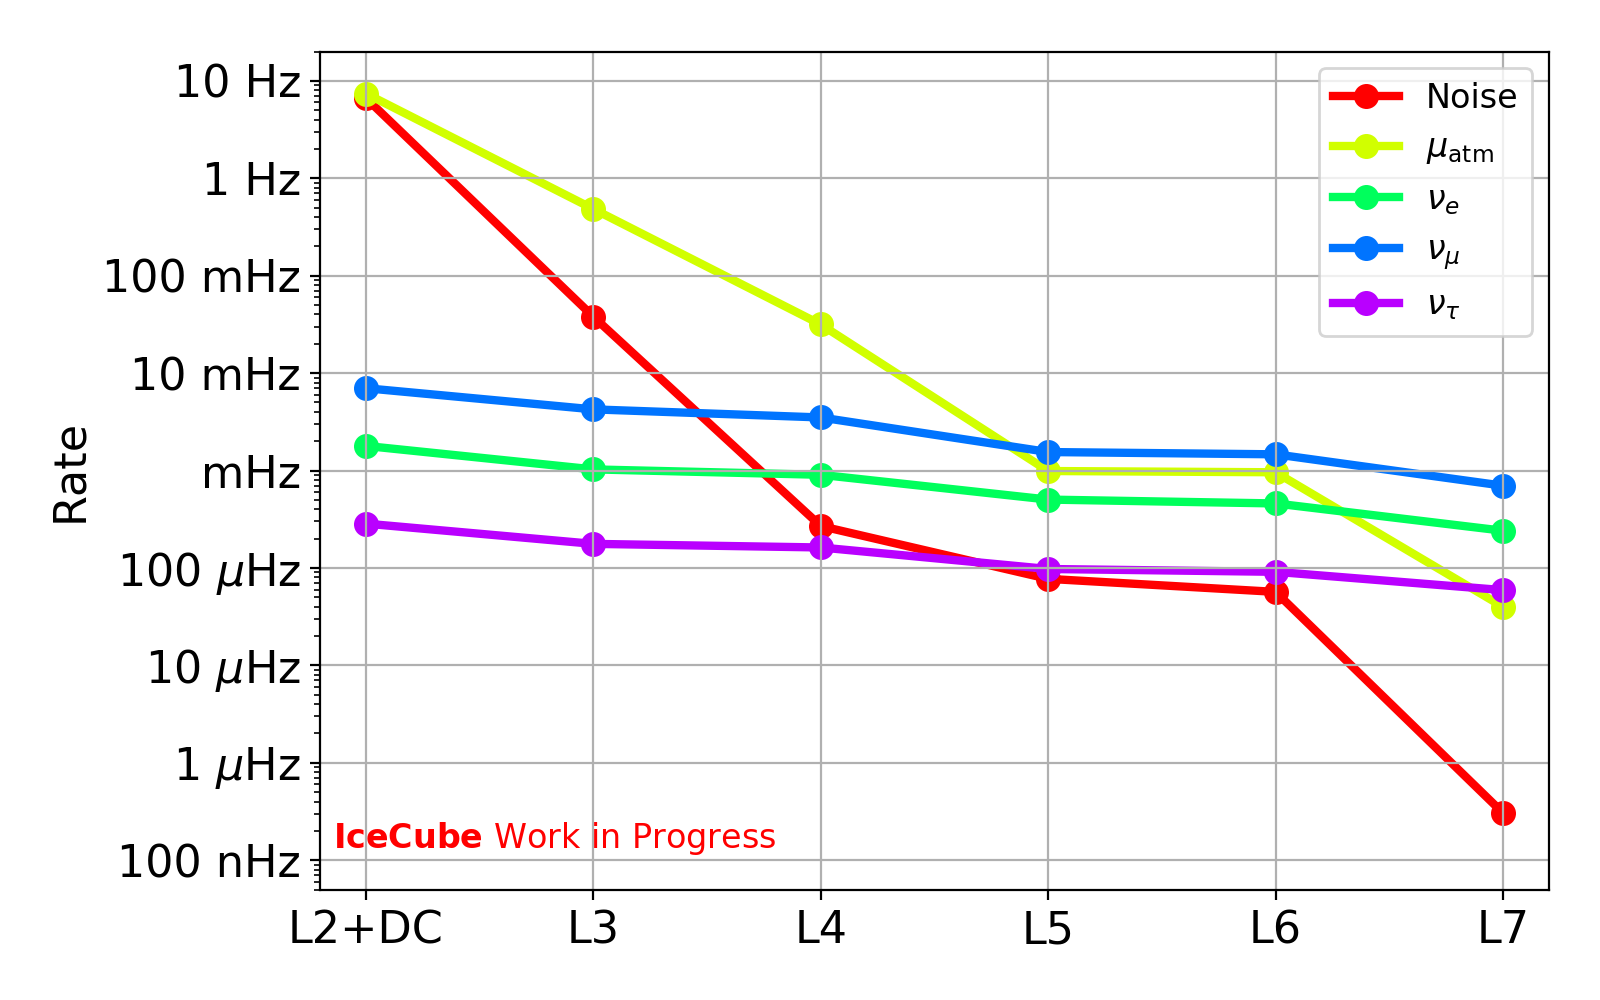
\includegraphics[width=.50\linewidth]{figures/OscNext_high_stats_event_selection_levels.png}
  \caption{Theoretical $\nu_{\mu}$ disappearance probability (left), and the rates of the IceCube neutrino sample after each selection level (LX) (right). L2+DC are the initial trigger and DeepCore filter, L3 and L4 are a basic and a multivariate-based background rejection step, respectively, L5 is a more advanced muon veto step, and L6/L7 are high-level reconstruction and final cuts to reduce muons and noise based on the results.}
  \label{fig:oscnext_sample_and_phasespace}
\end{figure}
Neutrino wave functions can be described by their mass eigenstates or their flavor eigenstates \cite{BILENKY1978225}, which are related as $\ket{\nu_\alpha} = \sum_kU^{3x3*}_{\alpha k}\ket{\nu_k}$, where $\ket{\nu_\alpha}$ are the flavor states with $\alpha=e,\mu,\tau$ and $\ket{\nu_k}$ the mass states with $k=1,2,3$. $U^{3x3}_{\alpha k}$ is the Pontecorvo-Maki-Nakagawa-Sakata (PMNS) matrix defining the mixing between mass and flavor states. The flavor states, which therefore are a superposition of the mass states \cite{PhysRevD.98.030001}, link the neutrinos to the charged leptons they interact with in weak CC interactions. A neutrino, produced in its flavor state, will propagate through space as its composing mass states. For (at least two) nonzero, non-equal neutrino masses, this leads to the observed phenomenon of neutrino flavor oscillations.
\begin{wrapfigure}{r}{0.5\textwidth}
  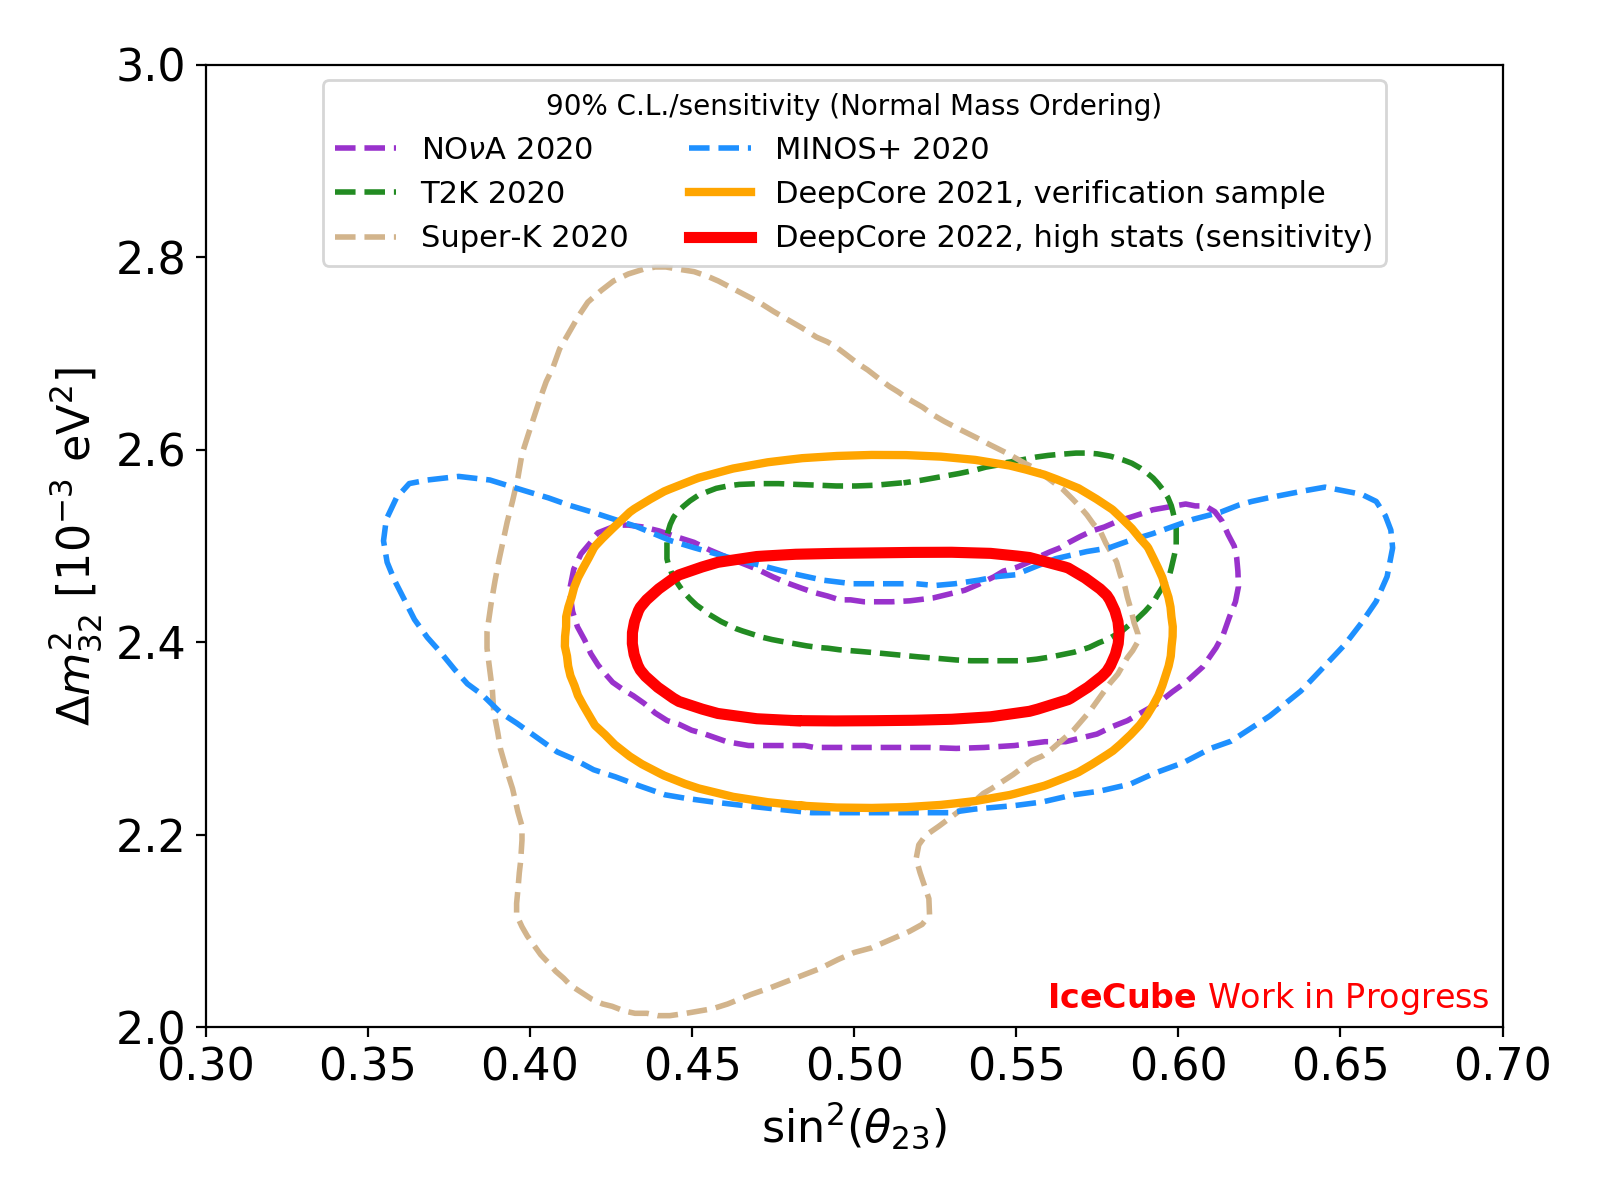
\includegraphics[width=0.5\textwidth]{figures/OscNext_numu_disappearance_sensitivity_public_v2.png}
  \caption{Latest results and expected sensitivity of IceCube DeepCore atmospheric neutrino oscillation analysis. \textit{DeepCore 2021, verification sample} is the golden (sub)-sample mentioned in the text, while \textit{DeepCore 2022, high stats} is the full sample.}
  \label{fig:oscnext_oscillations_results}
\end{wrapfigure}
By observing the flux of atmospheric neutrinos above energies of $5\,$GeV, IceCube has the ability to measure $U_{\mu3}$, $U_{\tau3}$, and $\Delta m^{2}_{32}$. For this purpose, an event selection was developed that reduces atmospheric muon and noise contamination down to sub-percent (negligible) level. \cref{fig:oscnext_sample_and_phasespace} shows the theoretical $\nu_{\mu}$ disappearance probability (left), and the expected rates for different event types for subsequent sample selection steps (right). IceCube is well suited to measure the first oscillation maximum that occurs in the 10\,GeV-50\,GeV region. By measuring the relative fluxes of neutrino flavors as a function of their reconstructed energies and arrival directions (related to cosine of incoming zenith angle), the parameters governing the oscillation pattern shown in \cref{fig:oscnext_sample_and_phasespace} can be measured. The flavor of the interacting neutrinos is inferred from the topology of the events, splitting the sample in track- and cascade-like parts. The analysis is performed using a binned maximum likelihood estimation to compare the data to Monte Carlo (MC) simulation for a specific hypothesis. \cref{fig:oscnext_oscillations_results} shows the latest results of the 8-year IceCube DeepCore neutrino oscillation analysis using a (sub-)sample of golden \footnote{Events containing \textit{direct photons} with minimal scattering along the light path.} events which constrained the atmospheric neutrino mixing parameters to be $\sin^2\theta_{23} = 0.505^{+0.051}_{-0.050}$ and $\Delta m^2_{32} = 2.41\pm0.084 \times 10^{-3}\mathrm{eV}^2$, assuming a normal mass ordering. Additionally shown is the expected sensitivity using the full sample, and the latest results from other experiments.


\vspace{-0.4cm}
\section{Heavy Neutral Lepton Search}

To incorporate the HNL into the original model, an additional heavy mass state and a sterile flavor state are added, turning the mixing relation into $\ket{\nu_\alpha} = \sum_kU^{4x4*}_{\alpha k}\ket{\nu_k}$, with $\alpha=e,\mu,\tau,s$ and $k=1,2,3,4$ and $U^{4x4}_{\alpha k}$ now being the extended 4x4 mixing matrix. The $\nu_s$ is a SM, right-handed singlet fermion and therefore not charged under the SM gauge groups. If the mass of the HNL is in the $\sim$\,GeV region, its production is kinematically accessible at atmospheric neutrino energies (10\,GeV-100\,GeV) and it can decay to SM particles. Because of its singlet property, its only way of interaction is through the weak interaction, inherited from the left-handed neutrinos via mixing \cite{Coloma:2020lgy}. The goal of this work is to probe the less constrained $|U_{\tau4}^2|$ mixing parameter, defining the $\tau$-sterile mixing space as shown in \cref{fig:hnl_limits}. Because of the phenomenon of neutrino oscillations, a significant part of the purely $\nu_{\mu/e}$ atmospheric neutrino flux oscillates into $\nu_\tau$ before it reaches the IceCube detector. The $\nu_\tau$ can interact in the ice, and produce the HNL in an up-scattering process. The HNL travels for a certain distance and then decays into lighter SM particles. The production and the decay can both produce a cascade-like light deposition, and if both happen inside the detector, they can be detected as a double-cascade. This type of signature can only be observed if sufficient light was produced at both the interaction and decay vertices. However, as can be seen from the decay BRs to the SM particles shown in \cref{fig:hnl_branching_ratios}, in most decays a neutrino carries away some energy, which is therefore not visible since neutrinos do not emit Cherenkov radiation. Additionally accounting for ice absorption length, optical detection efficiency and sparsity of the DOMs, the detection of both cascades is not always possible. Generally, if the energy of one of the cascades is too low, or the distance between the cascades is too short, the signature will be single-cascade-like. An example of the unique double-cascade-like event topology is shown in \cref{fig:low_energy_eventviews}.

\begin{wrapfigure}{r}{0.6\textwidth}
  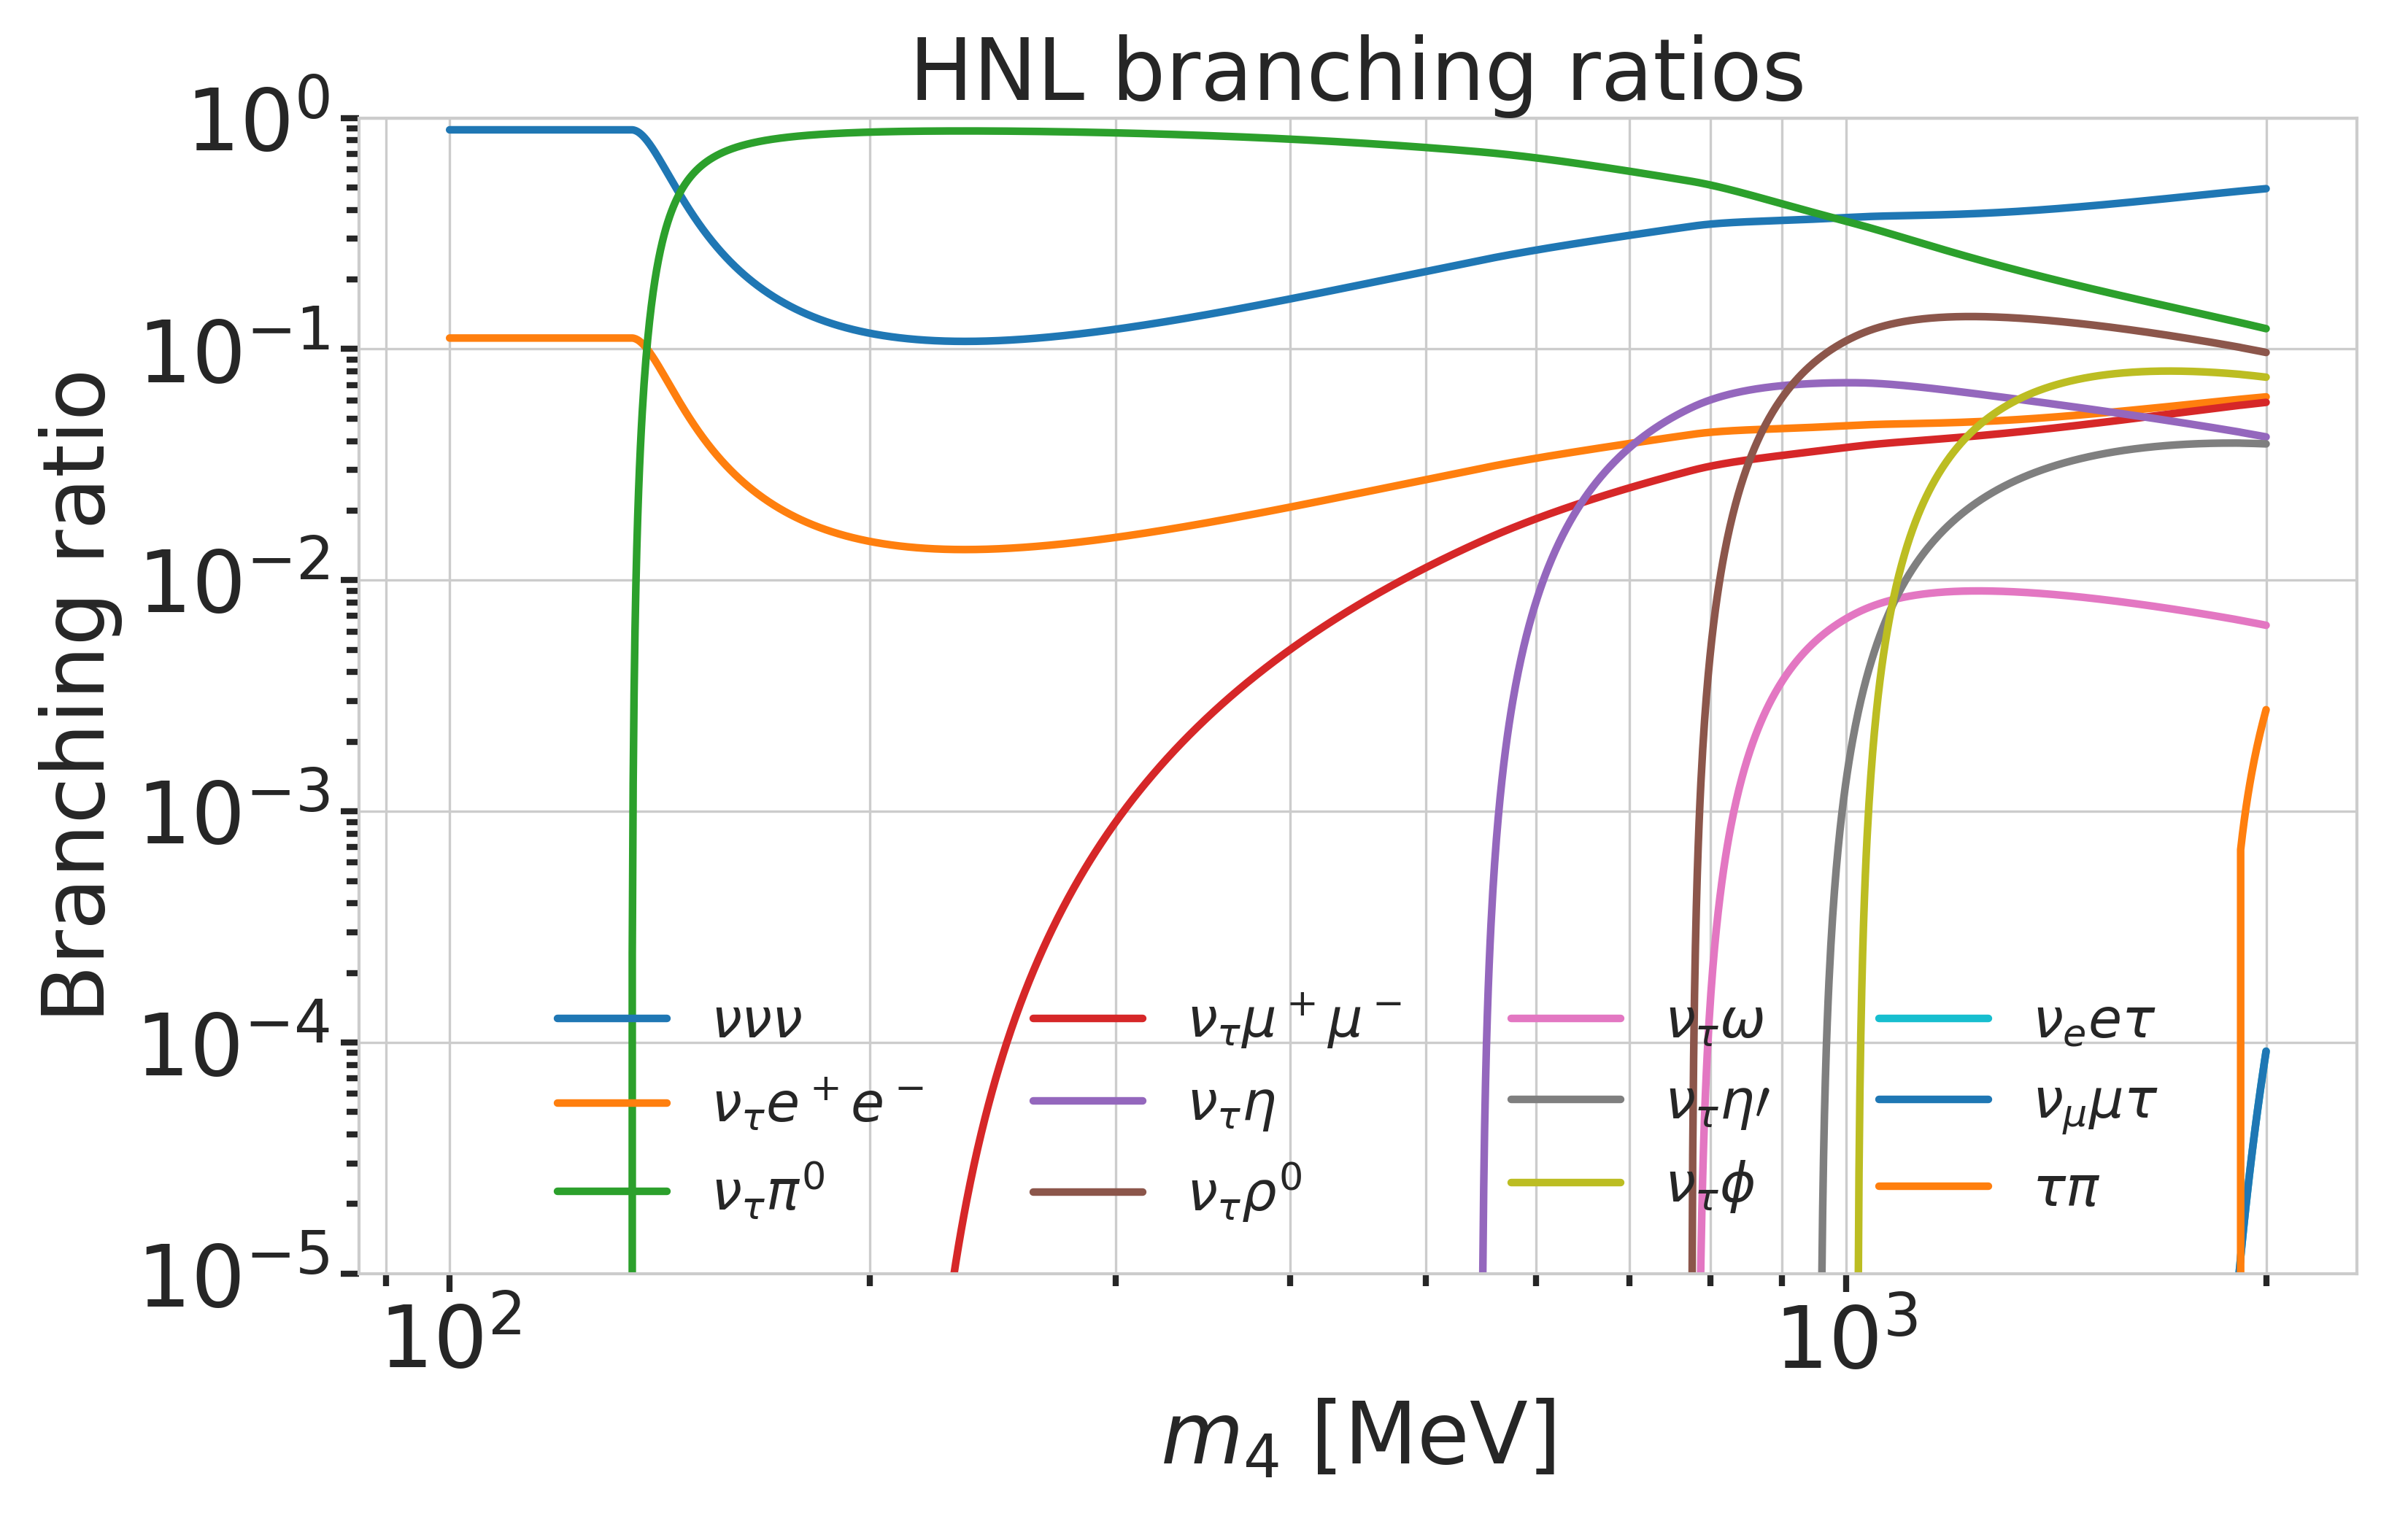
\includegraphics[width=0.6\textwidth]{figures/branching_ratios_log_up_to_2GeV.png}
  \caption{HNL decay branching ratios in IceCube calculated based on the results from \cite{Coloma:2020lgy}.}
  \label{fig:hnl_branching_ratios}
\end{wrapfigure}

To search for such events, we start from the same event selection used for the oscillation analysis described in \cref{sec:neutrino_oscillations}, which was developed to select atmospheric neutrino events in DeepCore by rejecting muons and noise. Since the HNL events are produced from the atmospheric neutrino flux, the event energies are very similar and starting from this selection is a valid first approach. The original analysis idea was to apply a specifically tailored reconstruction, assuming a double-cascade hypothesis, and then select them using a boosted decision tree (BDT) method, where the reconstructed double-cascade parameters were used as input. The reconstruction fits a double-cascade hypothesis by minimizing a Poisson likelihood, where the expected light, calculated from tabulated simulation, is compared to the observed light pattern. Isolating a double-cascade signal (S) region from the SM background (B) should lead to strong constraints in the tested mixing-mass space, but it turns out that isolating a pure signal region is a more challenging task than expected. The main problem is that many of the SM neutrino interactions look very similar to the double-cascade events because: 1) the energies are generally very low, which results in very few photons being emitted, and 2) the sparsity of the detector allows only a fraction of those to be detected. For the double-cascade events, the energy distribution of the second cascade is especially low since part of the energy is oftentimes being carried away by the invisible neutrino. As a result, most of the HNL events look like single cascades. On top of that, the total HNL rate is much smaller than the SM neutrino rate ($S/B\sim O(10^{-4})$). Since this simple cut\&count analysis approach does not work, a more sophisticated principle is envisioned. Similar to the standard neutrino oscillation analysis, the events will be separated in multiple particle identification (PID) bins, as well as bins in other reconstructed quantities. The exact binning scheme is not defined yet, but the idea is to use the shape of HNL signal distributions on top of the SM backgrounds in cascade/track/double-cascade bins to constrain the mixing parameter. \cref{fig:s_over_sqrt_B_HNL} shows the $S/\sqrt{B}$ distribution in the (oscillation analysis) cascade-like PID bin. Using this binning, which was not optimized for the HNL search, the observed signal already looks promising.

\begin{figure}[h!]
  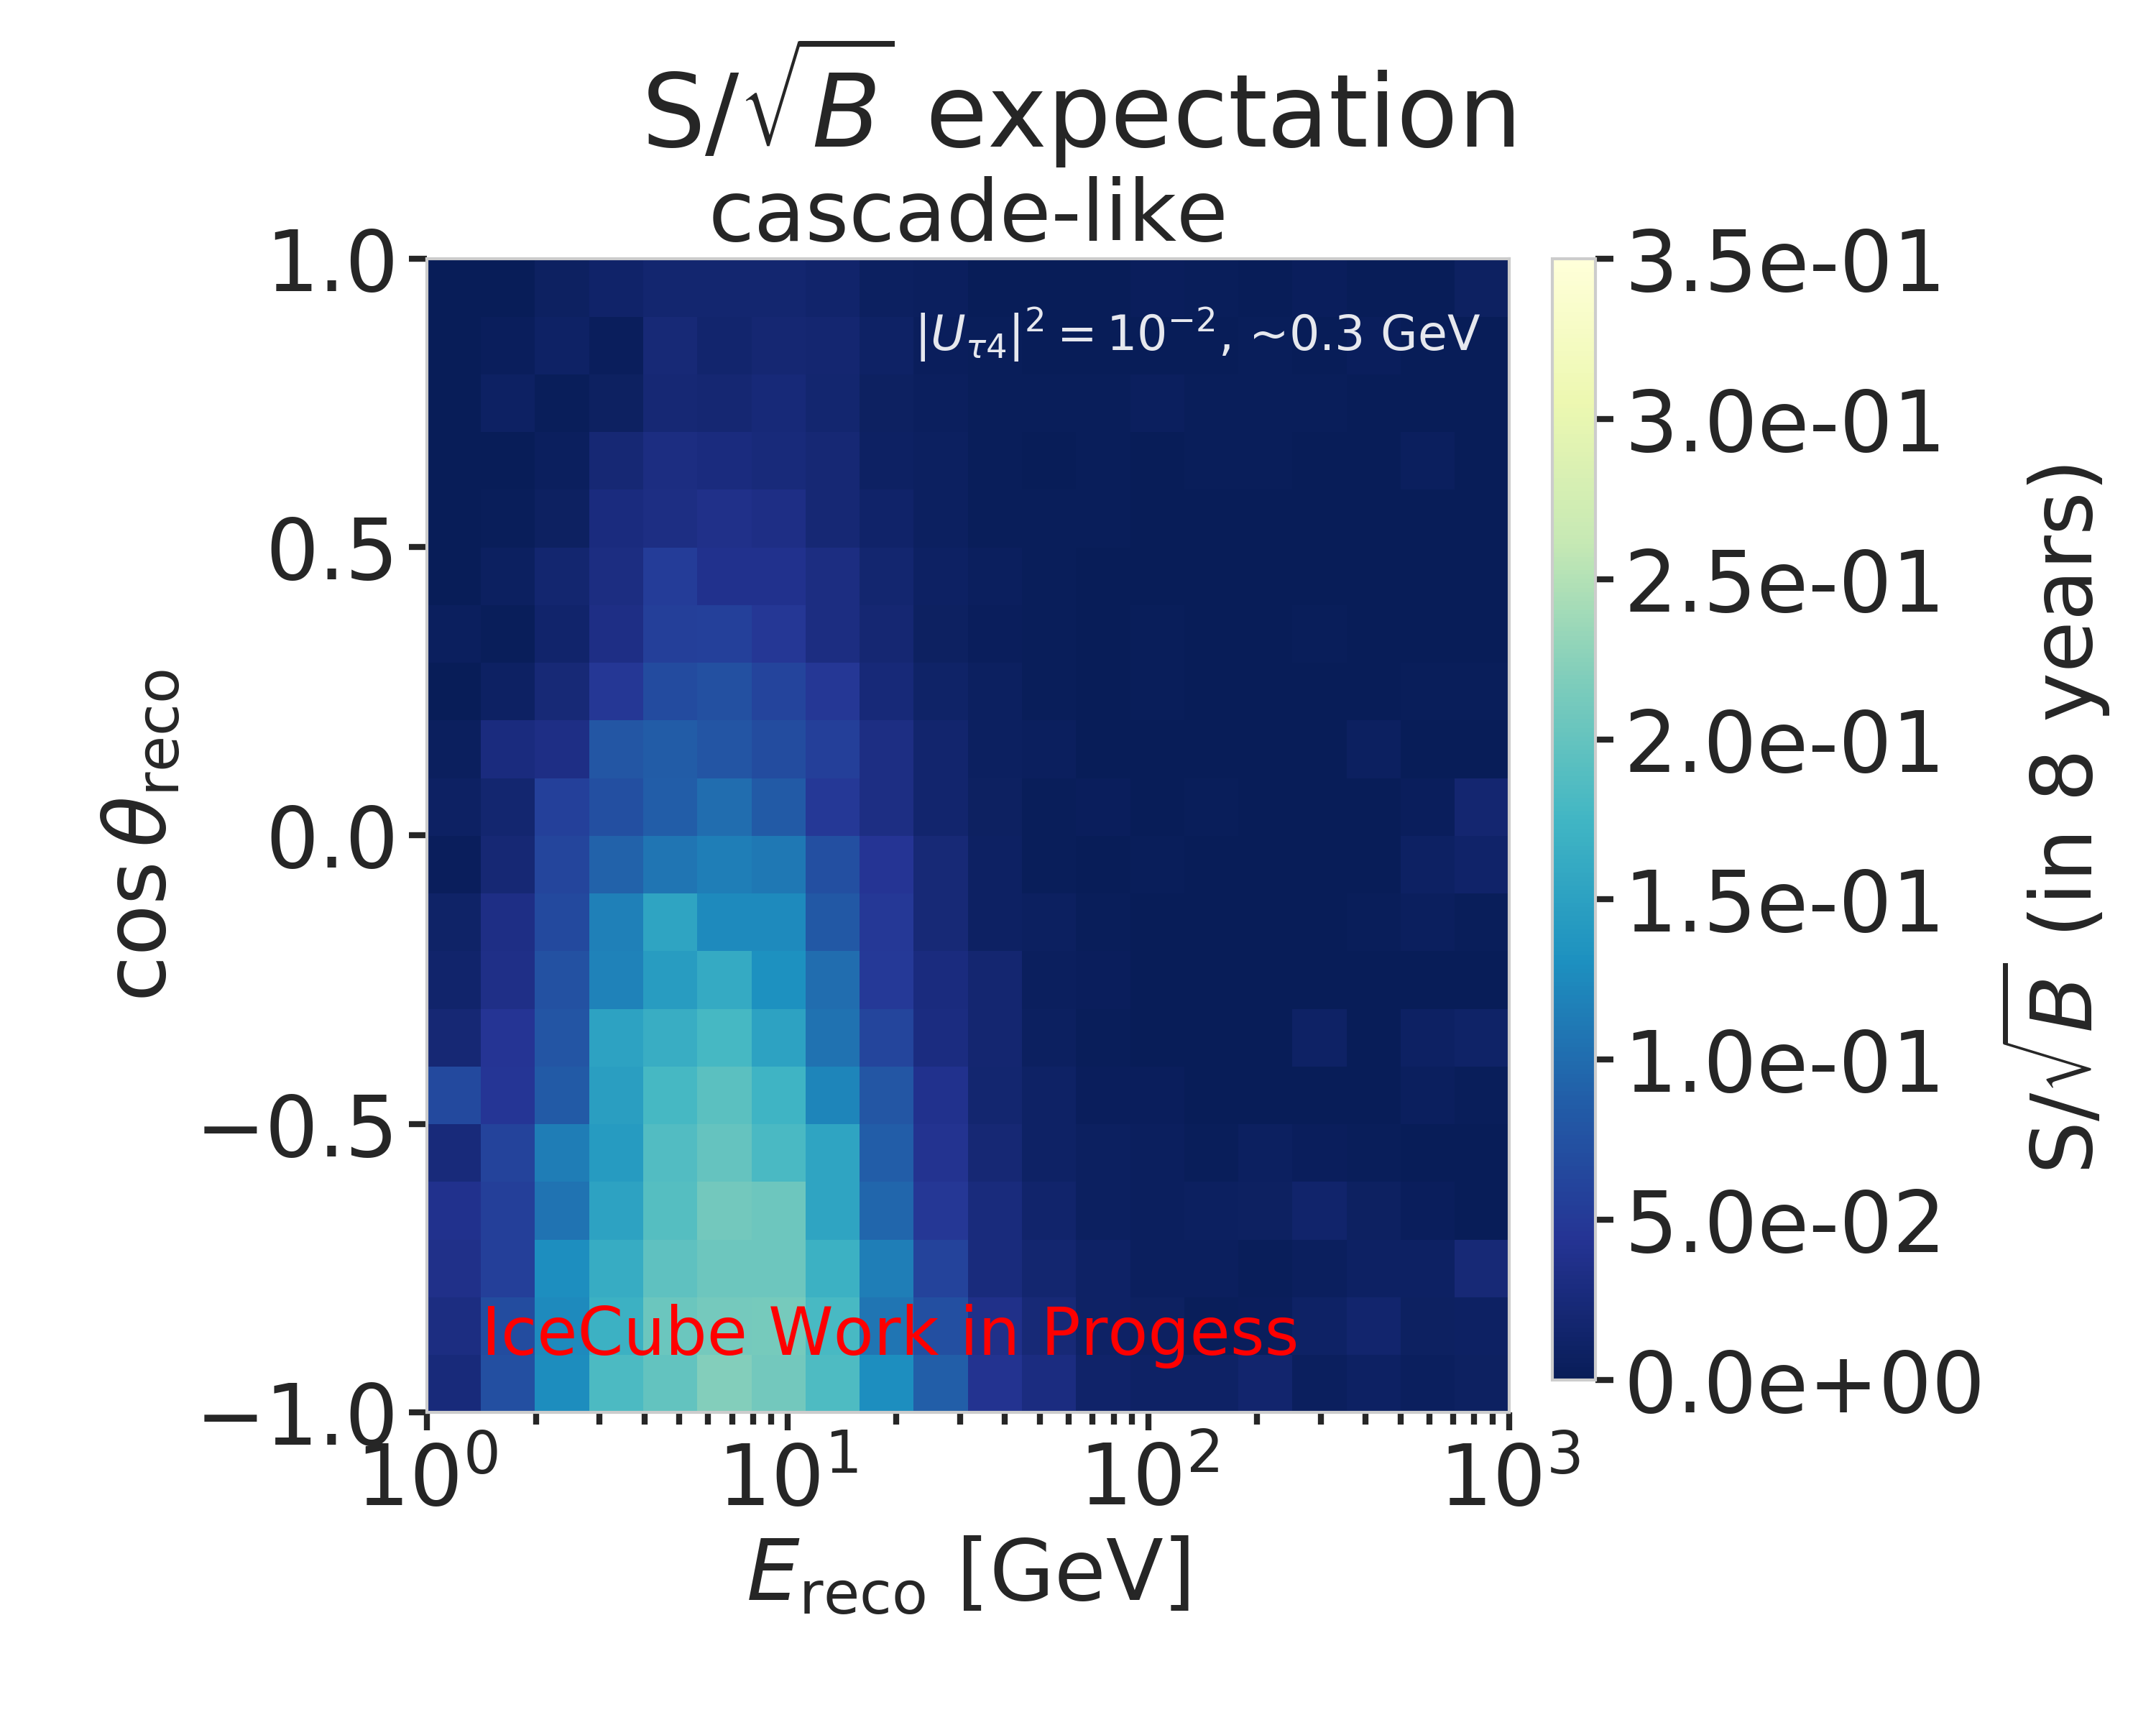
\includegraphics[trim = 0cm 0cm 7.15cm 2.0cm, clip, height=0.4\linewidth]{figures/2_d_S_over_sqrt(B)_taupede_reco_energy_taupede_reco_coszen_around_0.3_GeV_new.png}
  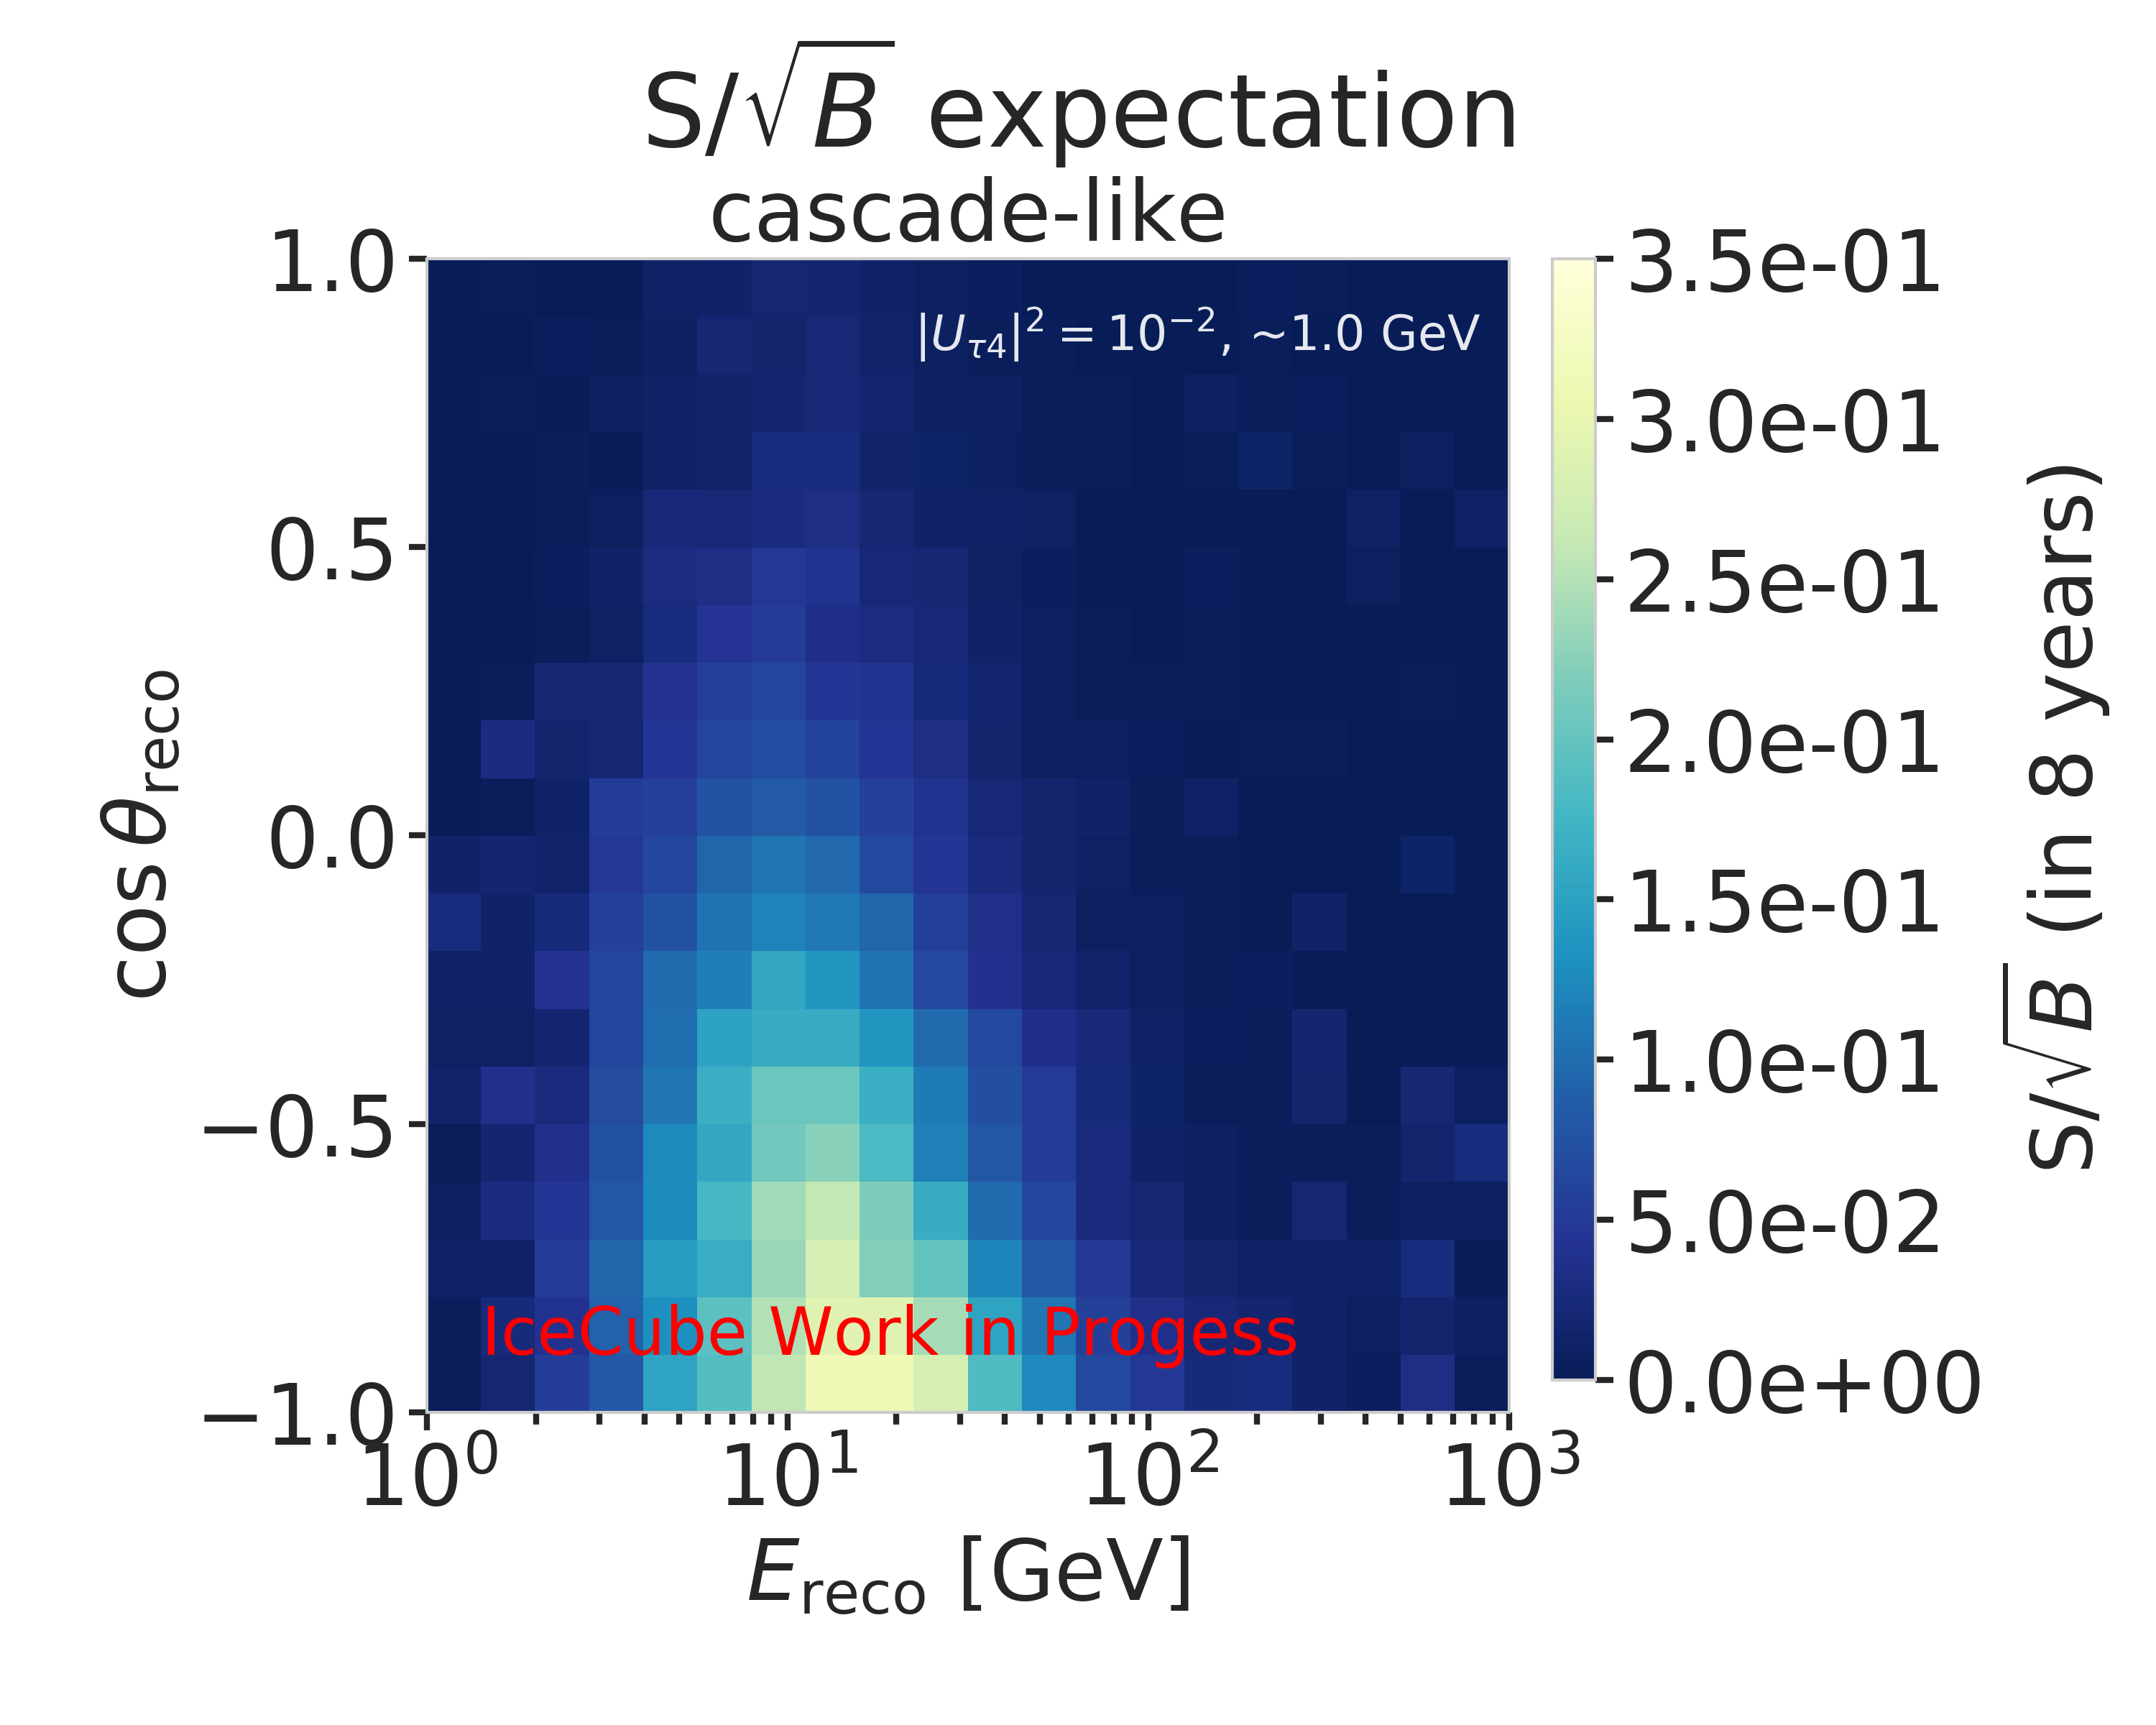
\includegraphics[trim = 0cm 0cm 0cm 2.0cm, clip, height=0.4\linewidth]{figures/2_d_S_over_sqrt(B)_taupede_reco_energy_taupede_reco_coszen_around_1.0_GeV_new.png}
  \caption{Signal (HNL) over square root of background (SM) in the cascade-like channel using the standard neutrino oscillation analysis binning for HNL masses of 0.3\,GeV (left), and 1.0\,GeV (right) and a mixing of $|U_{\tau4}^2|=10^{-2}$.}
  \label{fig:s_over_sqrt_B_HNL}
\end{figure}

With 8 years of IceCube DeepCore we are able to perform world-leading measurements of atmospheric neutrino oscillation parameters. The large flux of $\nu_\tau$ arriving at the detector offers the unique possibility for a search for HNLs. We have presented the progress of the search through up-scattering of $\nu_\tau$ and decay to SM particles. Work is ongoing for searching these events, utilizing both single- and double-cascade channels in order to maximize the expected signal-over-background.

\begingroup
    \scriptsize
    \setstretch{0.0}
    \bibliographystyle{JHEP}
    \bibliography{MyBibFile}
\endgroup


\end{document}  
